\section{Freestart collisions for 76-step SHA-1}
\label{sec:res_76}

This section gives the attack parameters for the 76-step freestart collision attack on \shaone.

\subsection{The differential path for most of the two first rounds}
\label{sec:app_diff_path}

We give a graphical representation of the differential path
used in our attack up to step 36 in \autoref{fig:diff_path}.
The meanings of the various symbols are defined
in \autoref{table:appbitconditions}.
The remainder of the path up to step 76 can easily
be determined by linerization of the step function, given the differences
in the message.

The additional message bit relations used in the attack for message words past $\expmess_{35}$ are given in \autoref{fig:msgbitrel76}, together with a
graphical representation in \autoref{fig:msgbitrel76_graph}.

%\begingroup
%\fontsize{8pt}{9pt}\selectfont
%\begin{verbbox}
%A-4 : ................................
%A-3 : ................................
%A-2 : .............................^+.
%A-1 : 0........................1.....+
%A0  : 10.0.....................0.0....     W 0 : ...........................+....
%A1  : .0.1................^.0....+....     W 1 : .....-.....................-++..
%A2  : ...^.-.........^.1....+....1.-.1     W 2 : -+..-+.....................+.-..
%A3  : .....-.1..^.1....+....1.-...^-.0     W 3 : ....+-........................+.
%A4  : .-.1...11.0.+....00-11..-.^..0+1     W 4 : +-.........................-....
%A5  : 1+.0.^.00^111.-.101-00.1..+.+1.0     W 5 : +.++.-.....................-+-..
%A6  : 00.-^-1-1--++++^01+0-.--.11.1.0-     W 6 : ..+-++.......................+..
%A7  : 1+.-^+-0-+10+-0^++-+1^1.0+..0.11     W 7 : +.+---.....................+-.-.
%A8  : +-.1..+-------------1-++11.-..+0     W 8 : ..-........................-....
%A9  : --+0.1.010.1000.10+-.0.100-1.10.     W 9 : ..+..+.....................-++..
%A10 : -10.1...1000111011001..111..10..     W10 : --+.+-.....................-.+..
%A11 : 1..-1...............10......1.^.     W11 : ....-+........................-.
%A12 : +.+..1..................^.......     W12 : -+.........................+....
%A13 : 0.+.10....................-....0     W13 : +.--.-.....................+--..
%A14 : ..+.........................0..1     W14 : ..-.-+.......................-..
%A15 : 1-..........................1.!.     W15 : +.-+++.....................+-...
%A16 : +..10.........................^.     W16 : -.-+.......................-....
%A17 : +.-1..........................!.     W17 : ............................-+..
%A18 : +...1..........................^     W18 : +.+-+......................-....
%A19 : .-..R...........................     W19 : ....-......................+-...
%A20 : -.RS............................     W20 : .++++......................+....
%A21 : -.-R............................     W21 : ....-......................+.+..
%A22 : -...s...........................     W22 : .-++.......................+....
%A23 : -.+.r...........................     W23 : -.+-+......................+-+..
%A24 : ....S...........................     W24 : --+.+...........................
%A25 : ..-.R...........................     W25 : -.++.........................+..
%A26 : -...S..........................^     W26 : .-.+-......................+....
%A27 : .--.r...........................     W27 : +.+-........................++..
%A28 : ..rSS...........................     W28 : .+..+...........................
%A29 : ...rr...........................     W29 : +.+-............................
%A30 : -...............................     W30 : -.+++......................+....
%A31 : -.s.............................     W31 : -..++......................+....
%A32 : ................................     W32 : -.+.............................
%A33 : ..R.............................     W33 : ................................
%A34 : ................................     W34 : ................................
%A35 : ................................     W35 : ..+.............................
%A36 : ................................
%\end{verbbox}
%\endgroup

\begin{figure}
\centering
\begin{tabular}{lcc}
$i$ & $\state_i$ & $\mess_i$\\
-4 & \nodiff\nodiff\nodiff\nodiff\nodiff\nodiff\nodiff\nodiff\nodiff\nodiff\nodiff\nodiff\nodiff\nodiff\nodiff\nodiff\nodiff\nodiff\nodiff\nodiff\nodiff\nodiff\nodiff\nodiff\nodiff\nodiff\nodiff\nodiff\nodiff\nodiff\nodiff\nodiff \\
-3 & \nodiff\nodiff\nodiff\nodiff\nodiff\nodiff\nodiff\nodiff\nodiff\nodiff\nodiff\nodiff\nodiff\nodiff\nodiff\nodiff\nodiff\nodiff\nodiff\nodiff\nodiff\nodiff\nodiff\nodiff\nodiff\nodiff\nodiff\nodiff\nodiff\nodiff\nodiff\nodiff \\
-2 & \nodiff\nodiff\nodiff\nodiff\nodiff\nodiff\nodiff\nodiff\nodiff\nodiff\nodiff\nodiff\nodiff\nodiff\nodiff\nodiff\nodiff\nodiff\nodiff\nodiff\nodiff\nodiff\nodiff\nodiff\nodiff\nodiff\nodiff\nodiff\nodiff\equaup$\monediffu$\nodiff \\
-1 & $\mnodiffz$\nodiff\nodiff\nodiff\nodiff\nodiff\nodiff\nodiff\nodiff\nodiff\nodiff\nodiff\nodiff\nodiff\nodiff\nodiff\nodiff\nodiff\nodiff\nodiff\nodiff\nodiff\nodiff\nodiff\nodiff$\mnodiffo$\nodiff\nodiff\nodiff\nodiff\nodiff$\monediffu$ \\
0 & $\mnodiffo$$\mnodiffz$\nodiff$\mnodiffz$\nodiff\nodiff\nodiff\nodiff\nodiff\nodiff\nodiff\nodiff\nodiff\nodiff\nodiff\nodiff\nodiff\nodiff\nodiff\nodiff\nodiff\nodiff\nodiff\nodiff\nodiff$\mnodiffz$\nodiff$\mnodiffz$\nodiff\nodiff\nodiff\nodiff     &  \nodiff\nodiff\nodiff\nodiff\nodiff\nodiff\nodiff\nodiff\nodiff\nodiff\nodiff\nodiff\nodiff\nodiff\nodiff\nodiff\nodiff\nodiff\nodiff\nodiff\nodiff\nodiff\nodiff\nodiff\nodiff\nodiff\nodiff$\monediffu$\nodiff\nodiff\nodiff\nodiff \\
1 & \nodiff$\mnodiffz$\nodiff$\mnodiffo$\nodiff\nodiff\nodiff\nodiff\nodiff\nodiff\nodiff\nodiff\nodiff\nodiff\nodiff\nodiff\nodiff\nodiff\nodiff\nodiff\equaup\nodiff$\mnodiffz$\nodiff\nodiff\nodiff\nodiff$\monediffu$\nodiff\nodiff\nodiff\nodiff     & \nodiff\nodiff\nodiff\nodiff\nodiff$\monediffd$\nodiff\nodiff\nodiff\nodiff\nodiff\nodiff\nodiff\nodiff\nodiff\nodiff\nodiff\nodiff\nodiff\nodiff\nodiff\nodiff\nodiff\nodiff\nodiff\nodiff\nodiff$\monediffd$$\monediffu$$\monediffu$\nodiff\nodiff \\
2 & \nodiff\nodiff\nodiff\equaup\nodiff$\monediffd$\nodiff\nodiff\nodiff\nodiff\nodiff\nodiff\nodiff\nodiff\nodiff\equaup\nodiff$\mnodiffo$\nodiff\nodiff\nodiff\nodiff$\monediffu$\nodiff\nodiff\nodiff\nodiff$\mnodiffo$\nodiff$\monediffd$\nodiff$\mnodiffo$     & $\monediffd$$\monediffu$\nodiff\nodiff$\monediffd$$\monediffu$\nodiff\nodiff\nodiff\nodiff\nodiff\nodiff\nodiff\nodiff\nodiff\nodiff\nodiff\nodiff\nodiff\nodiff\nodiff\nodiff\nodiff\nodiff\nodiff\nodiff\nodiff$\monediffu$\nodiff$\monediffd$\nodiff\nodiff \\
3 & \nodiff\nodiff\nodiff\nodiff\nodiff$\monediffd$\nodiff$\mnodiffo$\nodiff\nodiff\equaup\nodiff$\mnodiffo$\nodiff\nodiff\nodiff\nodiff$\monediffu$\nodiff\nodiff\nodiff\nodiff$\mnodiffo$\nodiff$\monediffd$\nodiff\nodiff\nodiff\equaup$\monediffd$\nodiff$\mnodiffz$     & \nodiff\nodiff\nodiff\nodiff$\monediffu$$\monediffd$\nodiff\nodiff\nodiff\nodiff\nodiff\nodiff\nodiff\nodiff\nodiff\nodiff\nodiff\nodiff\nodiff\nodiff\nodiff\nodiff\nodiff\nodiff\nodiff\nodiff\nodiff\nodiff\nodiff\nodiff$\monediffu$\nodiff \\
4 & \nodiff$\monediffd$\nodiff$\mnodiffo$\nodiff\nodiff\nodiff$\mnodiffo$$\mnodiffo$\nodiff$\mnodiffz$\nodiff$\monediffu$\nodiff\nodiff\nodiff\nodiff$\mnodiffz$$\mnodiffz$$\monediffd$$\mnodiffo$$\mnodiffo$\nodiff\nodiff$\monediffd$\nodiff\equaup\nodiff\nodiff$\mnodiffz$$\monediffu$$\mnodiffo$     & $\monediffu$$\monediffd$\nodiff\nodiff\nodiff\nodiff\nodiff\nodiff\nodiff\nodiff\nodiff\nodiff\nodiff\nodiff\nodiff\nodiff\nodiff\nodiff\nodiff\nodiff\nodiff\nodiff\nodiff\nodiff\nodiff\nodiff\nodiff$\monediffd$\nodiff\nodiff\nodiff\nodiff \\
5 & $\mnodiffo$$\monediffu$\nodiff$\mnodiffz$\nodiff\equaup\nodiff$\mnodiffz$$\mnodiffz$\equaup$\mnodiffo$$\mnodiffo$$\mnodiffo$\nodiff$\monediffd$\nodiff$\mnodiffo$$\mnodiffz$$\mnodiffo$$\monediffd$$\mnodiffz$$\mnodiffz$\nodiff$\mnodiffo$\nodiff\nodiff$\monediffu$\nodiff$\monediffu$$\mnodiffo$\nodiff$\mnodiffz$     & $\monediffu$\nodiff$\monediffu$$\monediffu$\nodiff$\monediffd$\nodiff\nodiff\nodiff\nodiff\nodiff\nodiff\nodiff\nodiff\nodiff\nodiff\nodiff\nodiff\nodiff\nodiff\nodiff\nodiff\nodiff\nodiff\nodiff\nodiff\nodiff$\monediffd$$\monediffu$$\monediffd$\nodiff\nodiff \\
6 & $\mnodiffz$$\mnodiffz$\nodiff$\monediffd$\equaup$\monediffd$$\mnodiffo$$\monediffd$$\mnodiffo$$\monediffd$$\monediffd$$\monediffu$$\monediffu$$\monediffu$$\monediffu$\equaup$\mnodiffz$$\mnodiffo$$\monediffu$$\mnodiffz$$\monediffd$\nodiff$\monediffd$$\monediffd$\nodiff$\mnodiffo$$\mnodiffo$\nodiff$\mnodiffo$\nodiff$\mnodiffz$$\monediffd$     & \nodiff\nodiff$\monediffu$$\monediffd$$\monediffu$$\monediffu$\nodiff\nodiff\nodiff\nodiff\nodiff\nodiff\nodiff\nodiff\nodiff\nodiff\nodiff\nodiff\nodiff\nodiff\nodiff\nodiff\nodiff\nodiff\nodiff\nodiff\nodiff\nodiff\nodiff$\monediffu$\nodiff\nodiff \\
7 & $\mnodiffo$$\monediffu$\nodiff$\monediffd$\equaup$\monediffu$$\monediffd$$\mnodiffz$$\monediffd$$\monediffu$$\mnodiffo$$\mnodiffz$$\monediffu$$\monediffd$$\mnodiffz$\equaup$\monediffu$$\monediffu$$\monediffd$$\monediffu$$\mnodiffo$\equaup$\mnodiffo$\nodiff$\mnodiffz$$\monediffu$\nodiff\nodiff$\mnodiffz$\nodiff$\mnodiffo$$\mnodiffo$     & $\monediffu$\nodiff$\monediffu$$\monediffd$$\monediffd$$\monediffd$\nodiff\nodiff\nodiff\nodiff\nodiff\nodiff\nodiff\nodiff\nodiff\nodiff\nodiff\nodiff\nodiff\nodiff\nodiff\nodiff\nodiff\nodiff\nodiff\nodiff\nodiff$\monediffu$$\monediffd$\nodiff$\monediffd$\nodiff \\
8 & $\monediffu$$\monediffd$\nodiff$\mnodiffo$\nodiff\nodiff$\monediffu$$\monediffd$$\monediffd$$\monediffd$$\monediffd$$\monediffd$$\monediffd$$\monediffd$$\monediffd$$\monediffd$$\monediffd$$\monediffd$$\monediffd$$\monediffd$$\mnodiffo$$\monediffd$$\monediffu$$\monediffu$$\mnodiffo$$\mnodiffo$\nodiff$\monediffd$\nodiff\nodiff$\monediffu$$\mnodiffz$     & \nodiff\nodiff$\monediffd$\nodiff\nodiff\nodiff\nodiff\nodiff\nodiff\nodiff\nodiff\nodiff\nodiff\nodiff\nodiff\nodiff\nodiff\nodiff\nodiff\nodiff\nodiff\nodiff\nodiff\nodiff\nodiff\nodiff\nodiff$\monediffd$\nodiff\nodiff\nodiff\nodiff \\
9 & $\monediffd$$\monediffd$$\monediffu$$\mnodiffz$\nodiff$\mnodiffo$\nodiff$\mnodiffz$$\mnodiffo$$\mnodiffz$\nodiff$\mnodiffo$$\mnodiffz$$\mnodiffz$$\mnodiffz$\nodiff$\mnodiffo$$\mnodiffz$$\monediffu$$\monediffd$\nodiff$\mnodiffz$\nodiff$\mnodiffo$$\mnodiffz$$\mnodiffz$$\monediffd$$\mnodiffo$\nodiff$\mnodiffo$$\mnodiffz$\nodiff     & \nodiff\nodiff$\monediffu$\nodiff\nodiff$\monediffu$\nodiff\nodiff\nodiff\nodiff\nodiff\nodiff\nodiff\nodiff\nodiff\nodiff\nodiff\nodiff\nodiff\nodiff\nodiff\nodiff\nodiff\nodiff\nodiff\nodiff\nodiff$\monediffd$$\monediffu$$\monediffu$\nodiff\nodiff \\
10 & $\monediffd$$\mnodiffo$$\mnodiffz$\nodiff$\mnodiffo$\nodiff\nodiff\nodiff$\mnodiffo$$\mnodiffz$$\mnodiffz$$\mnodiffz$$\mnodiffo$$\mnodiffo$$\mnodiffo$$\mnodiffz$$\mnodiffo$$\mnodiffo$$\mnodiffz$$\mnodiffz$$\mnodiffo$\nodiff\nodiff$\mnodiffo$$\mnodiffo$$\mnodiffo$\nodiff\nodiff$\mnodiffo$$\mnodiffz$\nodiff\nodiff     & $\monediffd$$\monediffd$$\monediffu$\nodiff$\monediffu$$\monediffd$\nodiff\nodiff\nodiff\nodiff\nodiff\nodiff\nodiff\nodiff\nodiff\nodiff\nodiff\nodiff\nodiff\nodiff\nodiff\nodiff\nodiff\nodiff\nodiff\nodiff\nodiff$\monediffd$\nodiff$\monediffu$\nodiff\nodiff \\
11 & $\mnodiffo$\nodiff\nodiff$\monediffd$$\mnodiffo$\nodiff\nodiff\nodiff\nodiff\nodiff\nodiff\nodiff\nodiff\nodiff\nodiff\nodiff\nodiff\nodiff\nodiff\nodiff$\mnodiffo$$\mnodiffz$\nodiff\nodiff\nodiff\nodiff\nodiff\nodiff$\mnodiffo$\nodiff\equaup\nodiff     & \nodiff\nodiff\nodiff\nodiff$\monediffd$$\monediffu$\nodiff\nodiff\nodiff\nodiff\nodiff\nodiff\nodiff\nodiff\nodiff\nodiff\nodiff\nodiff\nodiff\nodiff\nodiff\nodiff\nodiff\nodiff\nodiff\nodiff\nodiff\nodiff\nodiff\nodiff$\monediffd$\nodiff \\
12 & $\monediffu$\nodiff$\monediffu$\nodiff\nodiff$\mnodiffo$\nodiff\nodiff\nodiff\nodiff\nodiff\nodiff\nodiff\nodiff\nodiff\nodiff\nodiff\nodiff\nodiff\nodiff\nodiff\nodiff\nodiff\nodiff\equaup\nodiff\nodiff\nodiff\nodiff\nodiff\nodiff\nodiff     & $\monediffd$$\monediffu$\nodiff\nodiff\nodiff\nodiff\nodiff\nodiff\nodiff\nodiff\nodiff\nodiff\nodiff\nodiff\nodiff\nodiff\nodiff\nodiff\nodiff\nodiff\nodiff\nodiff\nodiff\nodiff\nodiff\nodiff\nodiff$\monediffu$\nodiff\nodiff\nodiff\nodiff \\
13 & $\mnodiffz$\nodiff$\monediffu$\nodiff$\mnodiffo$$\mnodiffz$\nodiff\nodiff\nodiff\nodiff\nodiff\nodiff\nodiff\nodiff\nodiff\nodiff\nodiff\nodiff\nodiff\nodiff\nodiff\nodiff\nodiff\nodiff\nodiff\nodiff$\monediffd$\nodiff\nodiff\nodiff\nodiff$\mnodiffz$     & $\monediffu$\nodiff$\monediffd$$\monediffd$\nodiff$\monediffd$\nodiff\nodiff\nodiff\nodiff\nodiff\nodiff\nodiff\nodiff\nodiff\nodiff\nodiff\nodiff\nodiff\nodiff\nodiff\nodiff\nodiff\nodiff\nodiff\nodiff\nodiff$\monediffu$$\monediffd$$\monediffd$\nodiff\nodiff \\
14 & \nodiff\nodiff$\monediffu$\nodiff\nodiff\nodiff\nodiff\nodiff\nodiff\nodiff\nodiff\nodiff\nodiff\nodiff\nodiff\nodiff\nodiff\nodiff\nodiff\nodiff\nodiff\nodiff\nodiff\nodiff\nodiff\nodiff\nodiff\nodiff$\mnodiffz$\nodiff\nodiff$\mnodiffo$     & \nodiff\nodiff$\monediffd$\nodiff$\monediffd$$\monediffu$\nodiff\nodiff\nodiff\nodiff\nodiff\nodiff\nodiff\nodiff\nodiff\nodiff\nodiff\nodiff\nodiff\nodiff\nodiff\nodiff\nodiff\nodiff\nodiff\nodiff\nodiff\nodiff\nodiff$\monediffd$\nodiff\nodiff \\
15 & $\mnodiffo$$\monediffd$\nodiff\nodiff\nodiff\nodiff\nodiff\nodiff\nodiff\nodiff\nodiff\nodiff\nodiff\nodiff\nodiff\nodiff\nodiff\nodiff\nodiff\nodiff\nodiff\nodiff\nodiff\nodiff\nodiff\nodiff\nodiff\nodiff$\mnodiffo$\nodiff\diffup\nodiff     & $\monediffu$\nodiff$\monediffd$$\monediffu$$\monediffu$$\monediffu$\nodiff\nodiff\nodiff\nodiff\nodiff\nodiff\nodiff\nodiff\nodiff\nodiff\nodiff\nodiff\nodiff\nodiff\nodiff\nodiff\nodiff\nodiff\nodiff\nodiff\nodiff$\monediffu$$\monediffd$\nodiff\nodiff\nodiff \\
16 & $\monediffu$\nodiff\nodiff$\mnodiffo$$\mnodiffz$\nodiff\nodiff\nodiff\nodiff\nodiff\nodiff\nodiff\nodiff\nodiff\nodiff\nodiff\nodiff\nodiff\nodiff\nodiff\nodiff\nodiff\nodiff\nodiff\nodiff\nodiff\nodiff\nodiff\nodiff\nodiff\equaup\nodiff     & $\monediffd$\nodiff$\monediffd$$\monediffu$\nodiff\nodiff\nodiff\nodiff\nodiff\nodiff\nodiff\nodiff\nodiff\nodiff\nodiff\nodiff\nodiff\nodiff\nodiff\nodiff\nodiff\nodiff\nodiff\nodiff\nodiff\nodiff\nodiff$\monediffd$\nodiff\nodiff\nodiff\nodiff \\
17 & $\monediffu$\nodiff$\monediffd$$\mnodiffo$\nodiff\nodiff\nodiff\nodiff\nodiff\nodiff\nodiff\nodiff\nodiff\nodiff\nodiff\nodiff\nodiff\nodiff\nodiff\nodiff\nodiff\nodiff\nodiff\nodiff\nodiff\nodiff\nodiff\nodiff\nodiff\nodiff\diffup\nodiff     & \nodiff\nodiff\nodiff\nodiff\nodiff\nodiff\nodiff\nodiff\nodiff\nodiff\nodiff\nodiff\nodiff\nodiff\nodiff\nodiff\nodiff\nodiff\nodiff\nodiff\nodiff\nodiff\nodiff\nodiff\nodiff\nodiff\nodiff\nodiff$\monediffd$$\monediffu$\nodiff\nodiff \\
18 & $\monediffu$\nodiff\nodiff\nodiff$\mnodiffo$\nodiff\nodiff\nodiff\nodiff\nodiff\nodiff\nodiff\nodiff\nodiff\nodiff\nodiff\nodiff\nodiff\nodiff\nodiff\nodiff\nodiff\nodiff\nodiff\nodiff\nodiff\nodiff\nodiff\nodiff\nodiff\nodiff\equaup     & $\monediffu$\nodiff$\monediffu$$\monediffd$$\monediffu$\nodiff\nodiff\nodiff\nodiff\nodiff\nodiff\nodiff\nodiff\nodiff\nodiff\nodiff\nodiff\nodiff\nodiff\nodiff\nodiff\nodiff\nodiff\nodiff\nodiff\nodiff\nodiff$\monediffd$\nodiff\nodiff\nodiff\nodiff \\
19 & \nodiff$\monediffd$\nodiff\nodiff\diffrightup\nodiff\nodiff\nodiff\nodiff\nodiff\nodiff\nodiff\nodiff\nodiff\nodiff\nodiff\nodiff\nodiff\nodiff\nodiff\nodiff\nodiff\nodiff\nodiff\nodiff\nodiff\nodiff\nodiff\nodiff\nodiff\nodiff\nodiff     & \nodiff\nodiff\nodiff\nodiff$\monediffd$\nodiff\nodiff\nodiff\nodiff\nodiff\nodiff\nodiff\nodiff\nodiff\nodiff\nodiff\nodiff\nodiff\nodiff\nodiff\nodiff\nodiff\nodiff\nodiff\nodiff\nodiff\nodiff$\monediffu$$\monediffd$\nodiff\nodiff\nodiff \\
20 & $\monediffd$\nodiff\diffrightup\diffrightupup\nodiff\nodiff\nodiff\nodiff\nodiff\nodiff\nodiff\nodiff\nodiff\nodiff\nodiff\nodiff\nodiff\nodiff\nodiff\nodiff\nodiff\nodiff\nodiff\nodiff\nodiff\nodiff\nodiff\nodiff\nodiff\nodiff\nodiff\nodiff     & \nodiff$\monediffu$$\monediffu$$\monediffu$$\monediffu$\nodiff\nodiff\nodiff\nodiff\nodiff\nodiff\nodiff\nodiff\nodiff\nodiff\nodiff\nodiff\nodiff\nodiff\nodiff\nodiff\nodiff\nodiff\nodiff\nodiff\nodiff\nodiff$\monediffu$\nodiff\nodiff\nodiff\nodiff \\
21 & $\monediffd$\nodiff$\monediffd$\diffrightup\nodiff\nodiff\nodiff\nodiff\nodiff\nodiff\nodiff\nodiff\nodiff\nodiff\nodiff\nodiff\nodiff\nodiff\nodiff\nodiff\nodiff\nodiff\nodiff\nodiff\nodiff\nodiff\nodiff\nodiff\nodiff\nodiff\nodiff\nodiff     & \nodiff\nodiff\nodiff\nodiff$\monediffd$\nodiff\nodiff\nodiff\nodiff\nodiff\nodiff\nodiff\nodiff\nodiff\nodiff\nodiff\nodiff\nodiff\nodiff\nodiff\nodiff\nodiff\nodiff\nodiff\nodiff\nodiff\nodiff$\monediffu$\nodiff$\monediffu$\nodiff\nodiff \\
22 & $\monediffd$\nodiff\nodiff\nodiff\equarightupup\nodiff\nodiff\nodiff\nodiff\nodiff\nodiff\nodiff\nodiff\nodiff\nodiff\nodiff\nodiff\nodiff\nodiff\nodiff\nodiff\nodiff\nodiff\nodiff\nodiff\nodiff\nodiff\nodiff\nodiff\nodiff\nodiff\nodiff     & \nodiff$\monediffd$$\monediffu$$\monediffu$\nodiff\nodiff\nodiff\nodiff\nodiff\nodiff\nodiff\nodiff\nodiff\nodiff\nodiff\nodiff\nodiff\nodiff\nodiff\nodiff\nodiff\nodiff\nodiff\nodiff\nodiff\nodiff\nodiff$\monediffu$\nodiff\nodiff\nodiff\nodiff \\
23 & $\monediffd$\nodiff$\monediffu$\nodiff\equarightup\nodiff\nodiff\nodiff\nodiff\nodiff\nodiff\nodiff\nodiff\nodiff\nodiff\nodiff\nodiff\nodiff\nodiff\nodiff\nodiff\nodiff\nodiff\nodiff\nodiff\nodiff\nodiff\nodiff\nodiff\nodiff\nodiff\nodiff     & $\monediffd$\nodiff$\monediffu$$\monediffd$$\monediffu$\nodiff\nodiff\nodiff\nodiff\nodiff\nodiff\nodiff\nodiff\nodiff\nodiff\nodiff\nodiff\nodiff\nodiff\nodiff\nodiff\nodiff\nodiff\nodiff\nodiff\nodiff\nodiff$\monediffu$$\monediffd$$\monediffu$\nodiff\nodiff \\
24 & \nodiff\nodiff\nodiff\nodiff\diffrightupup\nodiff\nodiff\nodiff\nodiff\nodiff\nodiff\nodiff\nodiff\nodiff\nodiff\nodiff\nodiff\nodiff\nodiff\nodiff\nodiff\nodiff\nodiff\nodiff\nodiff\nodiff\nodiff\nodiff\nodiff\nodiff\nodiff\nodiff     & $\monediffd$$\monediffd$$\monediffu$\nodiff$\monediffu$\nodiff\nodiff\nodiff\nodiff\nodiff\nodiff\nodiff\nodiff\nodiff\nodiff\nodiff\nodiff\nodiff\nodiff\nodiff\nodiff\nodiff\nodiff\nodiff\nodiff\nodiff\nodiff\nodiff\nodiff\nodiff\nodiff\nodiff \\
25 & \nodiff\nodiff$\monediffd$\nodiff\diffrightup\nodiff\nodiff\nodiff\nodiff\nodiff\nodiff\nodiff\nodiff\nodiff\nodiff\nodiff\nodiff\nodiff\nodiff\nodiff\nodiff\nodiff\nodiff\nodiff\nodiff\nodiff\nodiff\nodiff\nodiff\nodiff\nodiff\nodiff     & $\monediffd$\nodiff$\monediffu$$\monediffu$\nodiff\nodiff\nodiff\nodiff\nodiff\nodiff\nodiff\nodiff\nodiff\nodiff\nodiff\nodiff\nodiff\nodiff\nodiff\nodiff\nodiff\nodiff\nodiff\nodiff\nodiff\nodiff\nodiff\nodiff\nodiff$\monediffu$\nodiff\nodiff \\
26 & $\monediffd$\nodiff\nodiff\nodiff\diffrightupup\nodiff\nodiff\nodiff\nodiff\nodiff\nodiff\nodiff\nodiff\nodiff\nodiff\nodiff\nodiff\nodiff\nodiff\nodiff\nodiff\nodiff\nodiff\nodiff\nodiff\nodiff\nodiff\nodiff\nodiff\nodiff\nodiff\equaup     & \nodiff$\monediffd$\nodiff$\monediffu$$\monediffd$\nodiff\nodiff\nodiff\nodiff\nodiff\nodiff\nodiff\nodiff\nodiff\nodiff\nodiff\nodiff\nodiff\nodiff\nodiff\nodiff\nodiff\nodiff\nodiff\nodiff\nodiff\nodiff$\monediffu$\nodiff\nodiff\nodiff\nodiff \\
27 & \nodiff$\monediffd$$\monediffd$\nodiff\equarightup\nodiff\nodiff\nodiff\nodiff\nodiff\nodiff\nodiff\nodiff\nodiff\nodiff\nodiff\nodiff\nodiff\nodiff\nodiff\nodiff\nodiff\nodiff\nodiff\nodiff\nodiff\nodiff\nodiff\nodiff\nodiff\nodiff\nodiff     & $\monediffu$\nodiff$\monediffu$$\monediffd$\nodiff\nodiff\nodiff\nodiff\nodiff\nodiff\nodiff\nodiff\nodiff\nodiff\nodiff\nodiff\nodiff\nodiff\nodiff\nodiff\nodiff\nodiff\nodiff\nodiff\nodiff\nodiff\nodiff\nodiff$\monediffu$$\monediffu$\nodiff\nodiff \\
28 & \nodiff\nodiff\equarightup\diffrightupup\diffrightupup\nodiff\nodiff\nodiff\nodiff\nodiff\nodiff\nodiff\nodiff\nodiff\nodiff\nodiff\nodiff\nodiff\nodiff\nodiff\nodiff\nodiff\nodiff\nodiff\nodiff\nodiff\nodiff\nodiff\nodiff\nodiff\nodiff\nodiff     & \nodiff$\monediffu$\nodiff\nodiff$\monediffu$\nodiff\nodiff\nodiff\nodiff\nodiff\nodiff\nodiff\nodiff\nodiff\nodiff\nodiff\nodiff\nodiff\nodiff\nodiff\nodiff\nodiff\nodiff\nodiff\nodiff\nodiff\nodiff\nodiff\nodiff\nodiff\nodiff\nodiff \\
29 & \nodiff\nodiff\nodiff\equarightup\equarightup\nodiff\nodiff\nodiff\nodiff\nodiff\nodiff\nodiff\nodiff\nodiff\nodiff\nodiff\nodiff\nodiff\nodiff\nodiff\nodiff\nodiff\nodiff\nodiff\nodiff\nodiff\nodiff\nodiff\nodiff\nodiff\nodiff\nodiff    & $\monediffu$\nodiff$\monediffu$$\monediffd$\nodiff\nodiff\nodiff\nodiff\nodiff\nodiff\nodiff\nodiff\nodiff\nodiff\nodiff\nodiff\nodiff\nodiff\nodiff\nodiff\nodiff\nodiff\nodiff\nodiff\nodiff\nodiff\nodiff\nodiff\nodiff\nodiff\nodiff\nodiff \\
30 & $\monediffd$\nodiff\nodiff\nodiff\nodiff\nodiff\nodiff\nodiff\nodiff\nodiff\nodiff\nodiff\nodiff\nodiff\nodiff\nodiff\nodiff\nodiff\nodiff\nodiff\nodiff\nodiff\nodiff\nodiff\nodiff\nodiff\nodiff\nodiff\nodiff\nodiff\nodiff\nodiff     & $\monediffd$\nodiff$\monediffu$$\monediffu$$\monediffu$\nodiff\nodiff\nodiff\nodiff\nodiff\nodiff\nodiff\nodiff\nodiff\nodiff\nodiff\nodiff\nodiff\nodiff\nodiff\nodiff\nodiff\nodiff\nodiff\nodiff\nodiff\nodiff$\monediffu$\nodiff\nodiff\nodiff\nodiff \\
31 & $\monediffd$\nodiff\equarightupup\nodiff\nodiff\nodiff\nodiff\nodiff\nodiff\nodiff\nodiff\nodiff\nodiff\nodiff\nodiff\nodiff\nodiff\nodiff\nodiff\nodiff\nodiff\nodiff\nodiff\nodiff\nodiff\nodiff\nodiff\nodiff\nodiff\nodiff\nodiff\nodiff     & $\monediffd$\nodiff\nodiff$\monediffu$$\monediffu$\nodiff\nodiff\nodiff\nodiff\nodiff\nodiff\nodiff\nodiff\nodiff\nodiff\nodiff\nodiff\nodiff\nodiff\nodiff\nodiff\nodiff\nodiff\nodiff\nodiff\nodiff\nodiff$\monediffu$\nodiff\nodiff\nodiff\nodiff \\
32 & \nodiff\nodiff\nodiff\nodiff\nodiff\nodiff\nodiff\nodiff\nodiff\nodiff\nodiff\nodiff\nodiff\nodiff\nodiff\nodiff\nodiff\nodiff\nodiff\nodiff\nodiff\nodiff\nodiff\nodiff\nodiff\nodiff\nodiff\nodiff\nodiff\nodiff\nodiff\nodiff     & $\monediffd$\nodiff$\monediffu$\nodiff\nodiff\nodiff\nodiff\nodiff\nodiff\nodiff\nodiff\nodiff\nodiff\nodiff\nodiff\nodiff\nodiff\nodiff\nodiff\nodiff\nodiff\nodiff\nodiff\nodiff\nodiff\nodiff\nodiff\nodiff\nodiff\nodiff\nodiff\nodiff \\
33 & \nodiff\nodiff\diffrightup\nodiff\nodiff\nodiff\nodiff\nodiff\nodiff\nodiff\nodiff\nodiff\nodiff\nodiff\nodiff\nodiff\nodiff\nodiff\nodiff\nodiff\nodiff\nodiff\nodiff\nodiff\nodiff\nodiff\nodiff\nodiff\nodiff\nodiff\nodiff\nodiff     & \nodiff\nodiff\nodiff\nodiff\nodiff\nodiff\nodiff\nodiff\nodiff\nodiff\nodiff\nodiff\nodiff\nodiff\nodiff\nodiff\nodiff\nodiff\nodiff\nodiff\nodiff\nodiff\nodiff\nodiff\nodiff\nodiff\nodiff\nodiff\nodiff\nodiff\nodiff\nodiff \\
34 & \nodiff\nodiff\nodiff\nodiff\nodiff\nodiff\nodiff\nodiff\nodiff\nodiff\nodiff\nodiff\nodiff\nodiff\nodiff\nodiff\nodiff\nodiff\nodiff\nodiff\nodiff\nodiff\nodiff\nodiff\nodiff\nodiff\nodiff\nodiff\nodiff\nodiff\nodiff\nodiff     & \nodiff\nodiff\nodiff\nodiff\nodiff\nodiff\nodiff\nodiff\nodiff\nodiff\nodiff\nodiff\nodiff\nodiff\nodiff\nodiff\nodiff\nodiff\nodiff\nodiff\nodiff\nodiff\nodiff\nodiff\nodiff\nodiff\nodiff\nodiff\nodiff\nodiff\nodiff\nodiff \\
35 & \nodiff\nodiff\nodiff\nodiff\nodiff\nodiff\nodiff\nodiff\nodiff\nodiff\nodiff\nodiff\nodiff\nodiff\nodiff\nodiff\nodiff\nodiff\nodiff\nodiff\nodiff\nodiff\nodiff\nodiff\nodiff\nodiff\nodiff\nodiff\nodiff\nodiff\nodiff\nodiff     & \nodiff\nodiff$\monediffu$\nodiff\nodiff\nodiff\nodiff\nodiff\nodiff\nodiff\nodiff\nodiff\nodiff\nodiff\nodiff\nodiff\nodiff\nodiff\nodiff\nodiff\nodiff\nodiff\nodiff\nodiff\nodiff\nodiff\nodiff\nodiff\nodiff\nodiff\nodiff\nodiff \\
36 & \nodiff\nodiff\nodiff\nodiff\nodiff\nodiff\nodiff\nodiff\nodiff\nodiff\nodiff\nodiff\nodiff\nodiff\nodiff\nodiff\nodiff\nodiff\nodiff\nodiff\nodiff\nodiff\nodiff\nodiff\nodiff\nodiff\nodiff\nodiff\nodiff\nodiff\nodiff\nodiff \\
\end{tabular}
\caption{The differential path of the 76-step attack up to step 36.\label{fig:diff_path}}
\end{figure}



%TODO move to Notations
\begin{figure}
{\centering\small%
\begin{tabular}{c c}
  \toprule
  Symbol & Condition on ($\state$,$\diff\state$) \\
	\midrule
  \nodiff & $\state_t[i] = \diff\state_t[i]$  \\
  \onediff & $\state_t[i] \neq \diff\state_t[i]$  \\
  \onediffu & $\state_t[i] = 0$, \quad $\diff\state_t[i] = 1$  \\
  \onediffd & $\state_t[i] = 1$, \quad $\diff\state_t[i] = 0$  \\
  $\mnodiffz$ & $\state_t[i] = \diff\state_t[i] = 0$\\
  $\mnodiffo$ & $\state_t[i] = \diff\state_t[i] = 1$ \\
  \equaup & $\state_t[i] = \diff\state_t[i] = A_{t-1}[i]$ \\
  \diffup & $\state_t[i] = \diff\state_t[i] \neq A_{t-1}[i]$ \\
	\equarightup & $\state_t[i] = \diff\state_t[i] = (A_{t-1} \ggg 2)[i]$  \\
	\diffrightup & $\state_t[i] = \diff\state_t[i] \neq (A_{t-1} \ggg 2)[i]$  \\
	\equarightupup & $\state_t[i] = \diff\state_t[i] = (A_{t-2} \ggg 2)[i]$  \\
	\diffrightupup & $\state_t[i] = \diff\state_t[i] \neq (A_{t-2} \ggg 2)[i]$  \\
  \bottomrule
\end{tabular}\\}
\caption{Meaning of the bit difference symbols, for a symbol located on $\state_t[i]$. The same symbols are also used for $\expmess$, $\diff\expmess$.}\label{table:appbitconditions}
\end{figure}

%\clearpage
%\section{Message bit-relations for steps 36--75}
%\label{sec:app_msgbitrel}

\begingroup
\fontsize{8pt}{9pt}\selectfont
\begin{verbbox}
- W54[29] ^ W55[29] = 0
- W53[29] ^ W55[29] = 0
- W51[4] ^ W55[29] = 0
- W49[29] ^ W50[29] = 0
- W48[29] ^ W50[29] = 0
- W47[28] ^ W47[29] = 1
- W46[4] ^ W50[29] = 0
- W46[28] ^ W47[28] = 0
- W46[29] ^ W47[28] = 1
- W45[28] ^ W47[28] = 0
- W44[29] ^ W44[30] = 0
- W43[3] ^ W47[28] = 0
- W43[4] ^ W47[28] = 1
- W42[29] ^ W47[28] = 1
- W41[4] ^ W47[28] = 0
- W40[29] ^ W47[28] = 0
- W39[4] ^ W47[28] = 1
- W37[4] ^ W47[28] = 0
- W59[4] ^ W63[29] = 0
- W57[4] ^ W59[29] = 0
- W74[0] = 1
- W75[5] = 0
- W73[1] ^ W74[6] = 1
- W71[5] ^ W75[30] = 0
- W70[0] ^ W75[30] = 1
\end{verbbox}
\endgroup
\begin{figure}
\begin{center}
\begin{tabular}{l l l}
 $\expmess_{54}[29] \oplus \expmess_{55}[29] = 0$ & $\expmess_{53}[29] \oplus \expmess_{55}[29] = 0$ & $\expmess_{51}[4]  \oplus \expmess_{55}[29] = 0$\\
 $\expmess_{49}[29] \oplus \expmess_{50}[29] = 0$ & $\expmess_{48}[29] \oplus \expmess_{50}[29] = 0$ & $\expmess_{47}[28] \oplus \expmess_{47}[29] = 1$\\
 $\expmess_{46}[4]  \oplus \expmess_{50}[29] = 0$ & $\expmess_{46}[28] \oplus \expmess_{47}[28] = 0$ & $\expmess_{46}[29] \oplus \expmess_{47}[28] = 1$\\
 $\expmess_{45}[28] \oplus \expmess_{47}[28] = 0$ & $\expmess_{44}[29] \oplus \expmess_{44}[30] = 0$ & $\expmess_{43}[3]  \oplus \expmess_{47}[28] = 0$\\
 $\expmess_{43}[4]  \oplus \expmess_{47}[28] = 1$ & $\expmess_{42}[29] \oplus \expmess_{47}[28] = 1$ & $\expmess_{41}[4]  \oplus \expmess_{47}[28] = 0$\\
 $\expmess_{40}[29] \oplus \expmess_{47}[28] = 0$ & $\expmess_{39}[4]  \oplus \expmess_{47}[28] = 1$ & $\expmess_{37}[4]  \oplus \expmess_{47}[28] = 0$\\
 $\expmess_{59}[4]  \oplus \expmess_{63}[29] = 0$ & $\expmess_{57}[4]  \oplus \expmess_{59}[29] = 0$ & $\expmess_{74}[0] = 1$\\ 
 $\expmess_{75}[5] = 0$ & $\expmess_{73}[1]  \oplus \expmess_{74}[6] = 1$ & $\expmess_{71}[5]  \oplus \expmess_{75}[30] = 0$\\
 $\expmess_{70}[0]  \oplus \expmess_{75}[30] = 1$\\
\end{tabular}
\end{center}
  \caption{The message bit relations of the 76-step attack for steps 36--75.
  \label{fig:msgbitrel76}}
\end{figure}

\begingroup
\fontsize{8pt}{9pt}\selectfont
\begin{verbbox}
W36:	 . . . . . . . . . . . . . . . . . . . . . . . . . . . . . . . .
W37:	 . . . . . . . . . . . . . . . . . . . . . . . . . . . r . . . .
W38:	 . . . . . . . . . . . . . . . . . . . . . . . . . . . . . . . .
W39:	 . . . . . . . . . . . . . . . . . . . . . . . . . . . q . . . .
W40:	 . . p . . . . . . . . . . . . . . . . . . . . . . . . . . . . .
W41:	 . . . . . . . . . . . . . . . . . . . . . . . . . . . o . . . .
W42:	 . . n . . . . . . . . . . . . . . . . . . . . . . . . . . . . .
W43:	 . . . . . . . . . . . . . . . . . . . . . . . . . . . m l . . .
W44:	 . k k . . . . . . . . . . . . . . . . . . . . . . . . . . . . .
W45:	 . . . j . . . . . . . . . . . . . . . . . . . . . . . . . . . .
W46:	 . . i h . . . . . . . . . . . . . . . . . . . . . . . g . . . .
W47:	 . . F @ . . . . . . . . . . . . . . . . . . . . . . . . . . . .
W48:	 . . e . . . . . . . . . . . . . . . . . . . . . . . . . . . . .
W49:	 . . d . . . . . . . . . . . . . . . . . . . . . . . . . . . . .
W50:	 . . * . . . . . . . . . . . . . . . . . . . . . . . . . . . . .
W51:	 . . . . . . . . . . . . . . . . . . . . . . . . . . . c . . . .
W52:	 . . . . . . . . . . . . . . . . . . . . . . . . . . . . . . . .
W53:	 . . b . . . . . . . . . . . . . . . . . . . . . . . . . . . . .
W54:	 . . a . . . . . . . . . . . . . . . . . . . . . . . . . . . . .
W55:	 . . $ . . . . . . . . . . . . . . . . . . . . . . . . . . . . .
W56:	 . . . . . . . . . . . . . . . . . . . . . . . . . . . . . . . .
W57:	 . . . . . . . . . . . . . . . . . . . . . . . . . . . t . . . .
W58:	 . . . . . . . . . . . . . . . . . . . . . . . . . . . . . . . .
W59:	 . . t . . . . . . . . . . . . . . . . . . . . . . . . s . . . .
W60:	 . . . . . . . . . . . . . . . . . . . . . . . . . . . . . . . .
W61:	 . . . . . . . . . . . . . . . . . . . . . . . . . . . . . . . .
W62:	 . . . . . . . . . . . . . . . . . . . . . . . . . . . . . . . .
W63:	 . . s . . . . . . . . . . . . . . . . . . . . . . . . . . . . .
W64:	 . . . . . . . . . . . . . . . . . . . . . . . . . . . . . . . .
W65:	 . . . . . . . . . . . . . . . . . . . . . . . . . . . . . . . .
W66:	 . . . . . . . . . . . . . . . . . . . . . . . . . . . . . . . .
W67:	 . . . . . . . . . . . . . . . . . . . . . . . . . . . . . . . .
W68:	 . . . . . . . . . . . . . . . . . . . . . . . . . . . . . . . .
W69:	 . . . . . . . . . . . . . . . . . . . . . . . . . . . . . . . .
W70:	 . . . . . . . . . . . . . . . . . . . . . . . . . . . . . . . w
W71:	 . . . . . . . . . . . . . . . . . . . . . . . . . . v . . . . .
W72:	 . . . . . . . . . . . . . . . . . . . . . . . . . . . . . . . .
W73:	 . . . . . . . . . . . . . . . . . . . . . . . . . . . . . . u .
W74:	 . . . . . . . . . . . . . . . . . . . . . . . . . U . . . . . 1
W75:	 . % . . . . . . . . . . . . . . . . . . . . . . . . 0 . . . . .

@ = fhIjlMNopQr
* = deg
$ = abc
% = vW
\end{verbbox}
\endgroup

\begin{figure}[ht]
\centering
  \theverbbox
  \caption{The message bit-relations used in the attack for words $\expmess_{36}$ to $\expmess_{75}$ (graphical representation).
  A dot (``\texttt{.}'') means an absence of condition. A zero (``\texttt{0}'') or one (``\texttt{1}'') character represents a bit unconditionally set to 0 or 1.
  A pair of two identical letters $x$ means that the two bits have the same value. A pair of two
  letters $x$ and $X$ means that the two bits have different values.
  Non-alphanumeric symbols are used as shorthand for bit positions with more than one relation.
  \label{fig:msgbitrel76_graph}}
\end{figure}

\subsection{The neutral bits}
\label{sec:neutral_bits}
We give here the list of the neutral bits used in the 76-step attack.
There are fifty-one of them over the eight message words
$\expmess_{14}$ to $\expmess_{21}$, distributed as
follows:
\begin{itemize}
\item $\expmess_{14}$: 9 neutral bits at  bit positions (starting with the least significant bit (\emph{LSB}) at zero) 5,6,7,8,9,10,11,12,13
\item $\expmess_{15}$: 11 neutral bits at positions 5,6,7,8,9,10,11,12,13,14,16
\item $\expmess_{16}$: 8 neutral bits at positions 6,7,8,9,10,11,13,16
\item $\expmess_{17}$: 5 neutral bits at positions 10,11,12,13,19
\item $\expmess_{18}$: 2 neutral bits at positions 15,16
\item $\expmess_{19}$: 8 neutral bits at positions 6,7,8,9,10,11,12,14
\item $\expmess_{20}$: 5 neutral bits at positions 0,6,11,12,13
\item $\expmess_{21}$: 3 neutral bits at positions 11,16,17
\end{itemize}
We give a graphical representation of the repartition of these neutral bits in \autoref{fig:neutbits76}.

\begin{verbbox}
W14: ..................xxxxxxxxx.....
W15: ...............x.xxxxxxxxxx.....
W16: ...............x..x.xxxxxx......
W17: ............x.....xxxx..........
W18: ...............xx...............
W19: .................x.xxxxxxx......
W20: ..................xxx....x.....x
W21: ..............xx....x...........
\end{verbbox}

\begin{figure}
\centering
\begin{tabular}{l c}
$\expmess_{14}$: & \nodiff\nodiff\nodiff\nodiff\nodiff\nodiff\nodiff\nodiff\nodiff\nodiff\nodiff\nodiff\nodiff\nodiff\nodiff\nodiff\nodiff\nodiff\onediff\onediff\onediff\onediff\onediff\onediff\onediff\onediff\onediff\nodiff\nodiff\nodiff\nodiff\nodiff \\
$\expmess_{15}$: & \nodiff\nodiff\nodiff\nodiff\nodiff\nodiff\nodiff\nodiff\nodiff\nodiff\nodiff\nodiff\nodiff\nodiff\nodiff\onediff\nodiff\onediff\onediff\onediff\onediff\onediff\onediff\onediff\onediff\onediff\onediff\nodiff\nodiff\nodiff\nodiff\nodiff \\
$\expmess_{16}$: & \nodiff\nodiff\nodiff\nodiff\nodiff\nodiff\nodiff\nodiff\nodiff\nodiff\nodiff\nodiff\nodiff\nodiff\nodiff\onediff\nodiff\nodiff\onediff\nodiff\onediff\onediff\onediff\onediff\onediff\onediff\nodiff\nodiff\nodiff\nodiff\nodiff\nodiff \\
$\expmess_{17}$: & \nodiff\nodiff\nodiff\nodiff\nodiff\nodiff\nodiff\nodiff\nodiff\nodiff\nodiff\nodiff\onediff\nodiff\nodiff\nodiff\nodiff\nodiff\onediff\onediff\onediff\onediff\nodiff\nodiff\nodiff\nodiff\nodiff\nodiff\nodiff\nodiff\nodiff\nodiff \\
$\expmess_{18}$: & \nodiff\nodiff\nodiff\nodiff\nodiff\nodiff\nodiff\nodiff\nodiff\nodiff\nodiff\nodiff\nodiff\nodiff\nodiff\onediff\onediff\nodiff\nodiff\nodiff\nodiff\nodiff\nodiff\nodiff\nodiff\nodiff\nodiff\nodiff\nodiff\nodiff\nodiff\nodiff \\
$\expmess_{19}$: & \nodiff\nodiff\nodiff\nodiff\nodiff\nodiff\nodiff\nodiff\nodiff\nodiff\nodiff\nodiff\nodiff\nodiff\nodiff\nodiff\nodiff\onediff\nodiff\onediff\onediff\onediff\onediff\onediff\onediff\onediff\nodiff\nodiff\nodiff\nodiff\nodiff\nodiff \\
$\expmess_{20}$: & \nodiff\nodiff\nodiff\nodiff\nodiff\nodiff\nodiff\nodiff\nodiff\nodiff\nodiff\nodiff\nodiff\nodiff\nodiff\nodiff\nodiff\nodiff\onediff\onediff\onediff\nodiff\nodiff\nodiff\nodiff\onediff\nodiff\nodiff\nodiff\nodiff\nodiff\onediff \\
$\expmess_{21}$: & \nodiff\nodiff\nodiff\nodiff\nodiff\nodiff\nodiff\nodiff\nodiff\nodiff\nodiff\nodiff\nodiff\nodiff\onediff\onediff\nodiff\nodiff\nodiff\nodiff\onediff\nodiff\nodiff\nodiff\nodiff\nodiff\nodiff\nodiff\nodiff\nodiff\nodiff\nodiff \\
\end{tabular}
  \caption{The fifty-one neutral bits of the 76-step attack, using (with some abuse) a ``difference'' notation.
  A ``\nodiff'' (resp. ``\onediff'') symbol means the absence (resp. presence) of a neutral bit on the corresponding bit.
  The message words are (as usual) written left to right from MSB to LSB.
  \label{fig:neutbits76}}
\end{figure}

Not all of the neutral bits located on the same word (say $\expmess_{14}$) are neutral up to the same state word. Their repartition
in that respect is as follows
\begin{itemize}
	\item Bits neutral up to step 18 (excluded): $\expmess_{14}$[9,10,11,12,13], $\expmess_{15}$[14,16]
	\item Bits neutral up to step 19 (excluded): $\expmess_{14}$[5,6,7,8], $\expmess_{15}$[8,9,10,11,12,13], $\expmess_{16}$[13,16], $\expmess_{17}$[19]
	\item Bits neutral up to step 20 (excluded): $\expmess_{15}$[5,6,7], $\expmess_{16}$[9,10,11]
	\item Bits neutral up to step 21 (excluded): $\expmess_{16}$[6,7,8], $\expmess_{17}$[10,11,12,13], $\expmess_{18}$[15,16]
	\item Bits neutral up to step 23 (excluded): $\expmess_{19}$[9,10,11,12,14]
	\item Bits neutral up to step 24 (excluded): $\expmess_{19}$[6,7], $\expmess_{20}$[11,12], $\expmess_{21}$[16,17]
	\item Bits neutral up to step 25 (excluded): $\expmess_{19}$[8], $\expmess_{20}$[6,13], $\expmess_{21}$[11]
	\item Bits neutral up to step 26 (excluded): $\expmess_{20}$[0]
\end{itemize}
We also give a graphical representation of this repartition in \autoref{fig:neutbits76_2}.

\begin{verbbox}
A18:
W14 ..................xxxxx.........
W15 ...............x.x..............

A19:
W14 .......................xxxx.....
W15 ..................xxxxxx........
W16 ...............x..x.............
W17 ............x...................

A20:
W15........................xxx.....
W16....................xxx.........

A21:
W16.......................xxx......
W17..................xxxx..........
W18...............xx...............

A23:
W19.................x.xxxx.........

A24:
W19........................xx......
W20...................xx...........
W21..............xx................

A25:
W19.......................x........
W20..................x......x......
W21....................x...........

A26:
W20...............................x
\end{verbbox}

\begin{figure}
\centering
\begin{tabular}{l c}
$\state_{18}$ \\
$\expmess_{14}$: & \nodiff\nodiff\nodiff\nodiff\nodiff\nodiff\nodiff\nodiff\nodiff\nodiff\nodiff\nodiff\nodiff\nodiff\nodiff\nodiff\nodiff\nodiff\onediff\onediff\onediff\onediff\onediff\nodiff\nodiff\nodiff\nodiff\nodiff\nodiff\nodiff\nodiff\nodiff \\
$\expmess_{15}$: & \nodiff\nodiff\nodiff\nodiff\nodiff\nodiff\nodiff\nodiff\nodiff\nodiff\nodiff\nodiff\nodiff\nodiff\nodiff\onediff\nodiff\onediff\nodiff\nodiff\nodiff\nodiff\nodiff\nodiff\nodiff\nodiff\nodiff\nodiff\nodiff\nodiff\nodiff\nodiff \\

$\state_{19}$ \\
$\expmess_{14}$: & \nodiff\nodiff\nodiff\nodiff\nodiff\nodiff\nodiff\nodiff\nodiff\nodiff\nodiff\nodiff\nodiff\nodiff\nodiff\nodiff\nodiff\nodiff\nodiff\nodiff\nodiff\nodiff\nodiff\onediff\onediff\onediff\onediff\nodiff\nodiff\nodiff\nodiff\nodiff \\
$\expmess_{15}$: & \nodiff\nodiff\nodiff\nodiff\nodiff\nodiff\nodiff\nodiff\nodiff\nodiff\nodiff\nodiff\nodiff\nodiff\nodiff\nodiff\nodiff\nodiff\onediff\onediff\onediff\onediff\onediff\onediff\nodiff\nodiff\nodiff\nodiff\nodiff\nodiff\nodiff\nodiff \\
$\expmess_{16}$: & \nodiff\nodiff\nodiff\nodiff\nodiff\nodiff\nodiff\nodiff\nodiff\nodiff\nodiff\nodiff\nodiff\nodiff\nodiff\onediff\nodiff\nodiff\onediff\nodiff\nodiff\nodiff\nodiff\nodiff\nodiff\nodiff\nodiff\nodiff\nodiff\nodiff\nodiff\nodiff \\
$\expmess_{17}$: & \nodiff\nodiff\nodiff\nodiff\nodiff\nodiff\nodiff\nodiff\nodiff\nodiff\nodiff\nodiff\onediff\nodiff\nodiff\nodiff\nodiff\nodiff\nodiff\nodiff\nodiff\nodiff\nodiff\nodiff\nodiff\nodiff\nodiff\nodiff\nodiff\nodiff\nodiff\nodiff \\

$\state_{20}$ \\
$\expmess_{15}$: & \nodiff\nodiff\nodiff\nodiff\nodiff\nodiff\nodiff\nodiff\nodiff\nodiff\nodiff\nodiff\nodiff\nodiff\nodiff\nodiff\nodiff\nodiff\nodiff\nodiff\nodiff\nodiff\nodiff\nodiff\onediff\onediff\onediff\nodiff\nodiff\nodiff\nodiff\nodiff \\
$\expmess_{16}$: & \nodiff\nodiff\nodiff\nodiff\nodiff\nodiff\nodiff\nodiff\nodiff\nodiff\nodiff\nodiff\nodiff\nodiff\nodiff\nodiff\nodiff\nodiff\nodiff\nodiff\onediff\onediff\onediff\nodiff\nodiff\nodiff\nodiff\nodiff\nodiff\nodiff\nodiff\nodiff \\

$\state_{21}$\\
$\expmess_{16}$: & \nodiff\nodiff\nodiff\nodiff\nodiff\nodiff\nodiff\nodiff\nodiff\nodiff\nodiff\nodiff\nodiff\nodiff\nodiff\nodiff\nodiff\nodiff\nodiff\nodiff\nodiff\nodiff\nodiff\onediff\onediff\onediff\nodiff\nodiff\nodiff\nodiff\nodiff\nodiff \\
$\expmess_{17}$: & \nodiff\nodiff\nodiff\nodiff\nodiff\nodiff\nodiff\nodiff\nodiff\nodiff\nodiff\nodiff\nodiff\nodiff\nodiff\nodiff\nodiff\nodiff\onediff\onediff\onediff\onediff\nodiff\nodiff\nodiff\nodiff\nodiff\nodiff\nodiff\nodiff\nodiff\nodiff \\
$\expmess_{18}$: & \nodiff\nodiff\nodiff\nodiff\nodiff\nodiff\nodiff\nodiff\nodiff\nodiff\nodiff\nodiff\nodiff\nodiff\nodiff\onediff\onediff\nodiff\nodiff\nodiff\nodiff\nodiff\nodiff\nodiff\nodiff\nodiff\nodiff\nodiff\nodiff\nodiff\nodiff\nodiff \\

$\state_{23}$\\
$\expmess_{19}$: & \nodiff\nodiff\nodiff\nodiff\nodiff\nodiff\nodiff\nodiff\nodiff\nodiff\nodiff\nodiff\nodiff\nodiff\nodiff\nodiff\nodiff\onediff\nodiff\onediff\onediff\onediff\onediff\nodiff\nodiff\nodiff\nodiff\nodiff\nodiff\nodiff\nodiff\nodiff \\

$\state_{24}$\\
$\expmess_{19}$: & \nodiff\nodiff\nodiff\nodiff\nodiff\nodiff\nodiff\nodiff\nodiff\nodiff\nodiff\nodiff\nodiff\nodiff\nodiff\nodiff\nodiff\nodiff\nodiff\nodiff\nodiff\nodiff\nodiff\nodiff\onediff\onediff\nodiff\nodiff\nodiff\nodiff\nodiff\nodiff \\
$\expmess_{20}$: & \nodiff\nodiff\nodiff\nodiff\nodiff\nodiff\nodiff\nodiff\nodiff\nodiff\nodiff\nodiff\nodiff\nodiff\nodiff\nodiff\nodiff\nodiff\nodiff\onediff\onediff\nodiff\nodiff\nodiff\nodiff\nodiff\nodiff\nodiff\nodiff\nodiff\nodiff\nodiff \\
$\expmess_{21}$: & \nodiff\nodiff\nodiff\nodiff\nodiff\nodiff\nodiff\nodiff\nodiff\nodiff\nodiff\nodiff\nodiff\nodiff\onediff\onediff\nodiff\nodiff\nodiff\nodiff\nodiff\nodiff\nodiff\nodiff\nodiff\nodiff\nodiff\nodiff\nodiff\nodiff\nodiff\nodiff \\

$\state_{25}$\\
$\expmess_{19}$: & \nodiff\nodiff\nodiff\nodiff\nodiff\nodiff\nodiff\nodiff\nodiff\nodiff\nodiff\nodiff\nodiff\nodiff\nodiff\nodiff\nodiff\nodiff\nodiff\nodiff\nodiff\nodiff\nodiff\onediff\nodiff\nodiff\nodiff\nodiff\nodiff\nodiff\nodiff\nodiff \\
$\expmess_{20}$: & \nodiff\nodiff\nodiff\nodiff\nodiff\nodiff\nodiff\nodiff\nodiff\nodiff\nodiff\nodiff\nodiff\nodiff\nodiff\nodiff\nodiff\nodiff\onediff\nodiff\nodiff\nodiff\nodiff\nodiff\nodiff\onediff\nodiff\nodiff\nodiff\nodiff\nodiff\nodiff \\
$\expmess_{21}$: & \nodiff\nodiff\nodiff\nodiff\nodiff\nodiff\nodiff\nodiff\nodiff\nodiff\nodiff\nodiff\nodiff\nodiff\nodiff\nodiff\nodiff\nodiff\nodiff\nodiff\onediff\nodiff\nodiff\nodiff\nodiff\nodiff\nodiff\nodiff\nodiff\nodiff\nodiff\nodiff \\

$\state_{26}$\\
$\expmess_{20}$: & \nodiff\nodiff\nodiff\nodiff\nodiff\nodiff\nodiff\nodiff\nodiff\nodiff\nodiff\nodiff\nodiff\nodiff\nodiff\nodiff\nodiff\nodiff\nodiff\nodiff\nodiff\nodiff\nodiff\nodiff\nodiff\nodiff\nodiff\nodiff\nodiff\nodiff\nodiff\onediff \\
\end{tabular}
  \caption{The fifty-one neutral bits regrouped by the first state where they start to interact. A ``\onediff'' represents the presence
  of a neutral bit, and a ``\nodiff'' the absence thereof. The LSB position is the rightmost one.
  \label{fig:neutbits76_2}}
\end{figure}

Finally, on the implementation side, we show how the neutral bits are packed together inside the ``inter-snippet'' buffers (mentioned in \autoref{sec:part_sol}) in \autoref{fig:nb_packing76} and
\autoref{fig:nb_packing76_2}. These figures represent each of the two words of the buffers as thirty-two numbered coloured circles, one for each bit. The colours represent the original message word from which the
bit comes from, and the number is the bit position in this original word. For instance, in \autoref{fig:nb_packing76}, 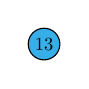
\begin{tikzpicture}[scale=0.67,transform shape]\draw[fill=Cerulean!85] (0,0) circle (.3) node{13};\end{tikzpicture}
is the value of the thirteenth bit (starting from zero) in some instance of $\expmess_{14}$ (\ie $\expmess_{14}[13]$); the fact that this circle is the leftmost one in the top sequence means that in the buffer, this information is stored as the MSB
of the first word.
One should note however that not all message bits shown in this packing are actually used as neutral bits. For instance, there is no neutral bit on $\expmess_{15}[15]$, yet this bit is included in \autoref{fig:nb_packing76}
as 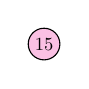
\begin{tikzpicture}[scale=0.67,transform shape]\draw[fill=Rhodamine!30] (0,0) circle (.3) node{15};\end{tikzpicture}. Although not including such non-neutral bits would save some space, it would make the storing process
more cumbersome and overall less efficient.

%\begin{figure}
%\begin{center}
%\begin{tikzpicture}[scale=0.67,transform shape]
%\draw[fill=Cerulean!65] (0,0) circle (.3) node{13};
%\draw[fill=Cerulean!65] (0.7,0) circle (.3) node{12};
%\draw[fill=Cerulean!65] (1.4,0) circle (.3) node{11};
%\draw[fill=Cerulean!65] (2.1,0) circle (.3) node{10};
%\draw[fill=Cerulean!65] (2.8,0) circle (.3) node{ 9};
%\draw[fill=Cerulean!65] (3.5,0) circle (.3) node{ 8};
%\draw[fill=Cerulean!65] (4.2,0) circle (.3) node{ 7};
%\draw[fill=Cerulean!65] (4.9,0) circle (.3) node{ 6};
%\draw[fill=Cerulean!65] (5.6,0) circle (.3) node{ 5};
%\draw[fill=WildStrawberry!30] (6.3,0) circle (.3) node{16};
%\draw[fill=WildStrawberry!30] (7.0,0) circle (.3) node{15};
%\draw[fill=WildStrawberry!30] (7.7,0) circle (.3) node{14};
%\draw[fill=WildStrawberry!30] (8.4,0) circle (.3) node{13};
%\draw[fill=WildStrawberry!30] (9.1,0) circle (.3) node{12};
%\draw[fill=WildStrawberry!30] (9.8,0) circle (.3) node{11};
%\draw[fill=WildStrawberry!30] (10.5,0) circle (.3) node{10};
%\draw[fill=WildStrawberry!30] (11.2,0) circle (.3) node{ 9};
%\draw[fill=WildStrawberry!30] (11.9,0) circle (.3) node{ 8};
%\draw[fill=WildStrawberry!30] (12.6,0) circle (.3) node{ 7};
%\draw[fill=WildStrawberry!30] (13.3,0) circle (.3) node{ 6};
%\draw[fill=WildStrawberry!30] (14.0,0) circle (.3) node{ 5};
%\draw[fill=BrickRed!65] (14.7,0) circle (.3) node{16};
%\draw[fill=BrickRed!65] (15.4,0) circle (.3) node{15};
%\draw[fill=BrickRed!65] (16.1,0) circle (.3) node{14};
%\draw[fill=BrickRed!65] (16.8,0) circle (.3) node{13};
%\draw[fill=BrickRed!65] (17.5,0) circle (.3) node{12};
%\draw[fill=BrickRed!65] (18.2,0) circle (.3) node{11};
%\draw[fill=BrickRed!65] (18.9,0) circle (.3) node{10};
%\draw[fill=BrickRed!65] (19.6,0) circle (.3) node{ 9};
%\draw[fill=BrickRed!65] (20.3,0) circle (.3) node{ 8};
%\draw[fill=BrickRed!65] (21.0,0) circle (.3) node{ 7};
%\draw[fill=BrickRed!65] (21.7,0) circle (.3) node{ 6};
%\draw[fill=YellowOrange!65] (0,-1) circle (.3) node{13};
%\draw[fill=YellowOrange!65] (0.7,-1) circle (.3) node{12};
%\draw[fill=YellowOrange!65] (1.4,-1) circle (.3) node{11};
%\draw[fill=YellowOrange!65] (2.1,-1) circle (.3) node{10};
%\draw[fill=YellowOrange!65] (2.8,-1) circle (.3) node{ 9};
%\draw[fill=YellowOrange!65] (3.5,-1) circle (.3) node{ 8};
%\draw[fill=YellowOrange!65] (4.2,-1) circle (.3) node{ 7};
%\draw[fill=YellowOrange!65] (4.9,-1) circle (.3) node{ 6};
%\draw[fill=YellowOrange!65] (5.6,-1) circle (.3) node{ 5};
%\draw[fill=LimeGreen!30] (6.3,-1) circle (.3) node{16};
%\draw[fill=LimeGreen!30] (7.0,-1) circle (.3) node{15};
%\draw[fill=LimeGreen!30] (7.7,-1) circle (.3) node{14};
%\draw[fill=LimeGreen!30] (8.4,-1) circle (.3) node{13};
%\draw[fill=LimeGreen!30] (9.1,-1) circle (.3) node{12};
%\draw[fill=LimeGreen!30] (9.8,-1) circle (.3) node{11};
%\draw[fill=LimeGreen!30] (10.5,-1) circle (.3) node{10};
%\draw[fill=LimeGreen!30] (11.2,-1) circle (.3) node{ 9};
%\draw[fill=LimeGreen!30] (11.9,-1) circle (.3) node{ 8};
%\draw[fill=LimeGreen!30] (12.6,-1) circle (.3) node{ 7};
%\draw[fill=LimeGreen!30] (13.3,-1) circle (.3) node{ 6};
%\draw[fill=LimeGreen!30] (14.0,-1) circle (.3) node{ 5};
%\draw[fill=Fuchsia!60] (14.7,-1) circle (.3) node{16};
%\draw[fill=Fuchsia!60] (15.4,-1) circle (.3) node{15};
%\draw[fill=Fuchsia!60] (16.1,-1) circle (.3) node{14};
%\draw[fill=Fuchsia!60] (16.8,-1) circle (.3) node{13};
%\draw[fill=Fuchsia!60] (17.5,-1) circle (.3) node{12};
%\draw[fill=Fuchsia!60] (18.2,-1) circle (.3) node{11};
%\draw[fill=Fuchsia!60] (18.9,-1) circle (.3) node{10};
%\draw[fill=Fuchsia!60] (19.6,-1) circle (.3) node{ 9};
%\draw[fill=Fuchsia!60] (20.3,-1) circle (.3) node{ 8};
%\draw[fill=Fuchsia!60] (21.0,-1) circle (.3) node{ 7};
%\draw[fill=Fuchsia!60] (21.7,-1) circle (.3) node{ 6};
%\end{tikzpicture}
%\end{center}
%\end{figure}

%\begin{verbbox}[\vspace{1mm}]
%For steps A18--21
%Word 1: W14 + W15 + W16 (32 bits)
%|<13..5>||<16.....5>||<16....6>|
%xxxxxxxxxx.xxxxxxxxxxx..x.xxxxxx
%Word 2: W17 + W18 (12 bits)
%|<19..10>||<16,15>/base sol id |
%x.....xxxxxx--------------------
%
%
%
%For steps A23--26
%Word 1: W21 + W19 + W20 (30 bits + 2 padding)
%\<17.11>||<14..6>||<13.......0>|
%~~xx....xx.xxxxxxxxxx....x.....x
%Word 2:
%            |	ext  sol id      |
%~~~~~~~~~~~~--------------------
%\end{verbbox}

\begin{figure}[!htb]
\begin{center}
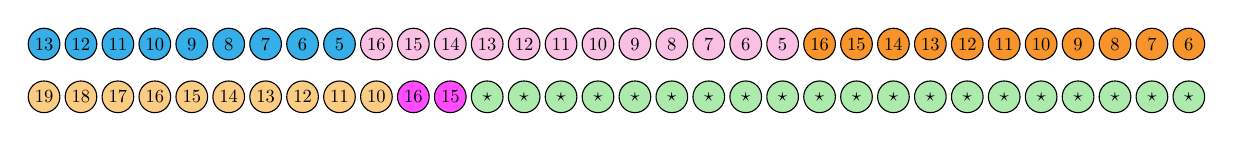
\begin{tikzpicture}[scale=0.67,transform shape]
\draw[fill=Cerulean!85] (0,0) circle (.3) node{13};
\draw[fill=Cerulean!85] (0.7,0) circle (.3) node{12};
\draw[fill=Cerulean!85] (1.4,0) circle (.3) node{11};
\draw[fill=Cerulean!85] (2.1,0) circle (.3) node{10};
\draw[fill=Cerulean!85] (2.8,0) circle (.3) node{ 9};
\draw[fill=Cerulean!85] (3.5,0) circle (.3) node{ 8};
\draw[fill=Cerulean!85] (4.2,0) circle (.3) node{ 7};
\draw[fill=Cerulean!85] (4.9,0) circle (.3) node{ 6};
\draw[fill=Cerulean!85] (5.6,0) circle (.3) node{ 5};
\draw[fill=Rhodamine!30] (6.3,0) circle (.3) node{16};
\draw[fill=Rhodamine!30] (7.0,0) circle (.3) node{15};
\draw[fill=Rhodamine!30] (7.7,0) circle (.3) node{14};
\draw[fill=Rhodamine!30] (8.4,0) circle (.3) node{13};
\draw[fill=Rhodamine!30] (9.1,0) circle (.3) node{12};
\draw[fill=Rhodamine!30] (9.8,0) circle (.3) node{11};
\draw[fill=Rhodamine!30] (10.5,0) circle (.3) node{10};
\draw[fill=Rhodamine!30] (11.2,0) circle (.3) node{ 9};
\draw[fill=Rhodamine!30] (11.9,0) circle (.3) node{ 8};
\draw[fill=Rhodamine!30] (12.6,0) circle (.3) node{ 7};
\draw[fill=Rhodamine!30] (13.3,0) circle (.3) node{ 6};
\draw[fill=Rhodamine!30] (14.0,0) circle (.3) node{ 5};
\draw[fill=BurntOrange!85] (14.7,0) circle (.3) node{16};
\draw[fill=BurntOrange!85] (15.4,0) circle (.3) node{15};
\draw[fill=BurntOrange!85] (16.1,0) circle (.3) node{14};
\draw[fill=BurntOrange!85] (16.8,0) circle (.3) node{13};
\draw[fill=BurntOrange!85] (17.5,0) circle (.3) node{12};
\draw[fill=BurntOrange!85] (18.2,0) circle (.3) node{11};
\draw[fill=BurntOrange!85] (18.9,0) circle (.3) node{10};
\draw[fill=BurntOrange!85] (19.6,0) circle (.3) node{ 9};
\draw[fill=BurntOrange!85] (20.3,0) circle (.3) node{ 8};
\draw[fill=BurntOrange!85] (21.0,0) circle (.3) node{ 7};
\draw[fill=BurntOrange!85] (21.7,0) circle (.3) node{ 6};
\draw[fill=YellowOrange!45] (0,-1) circle (.3) node{19};
\draw[fill=YellowOrange!45] (0.7,-1) circle (.3) node{18};
\draw[fill=YellowOrange!45] (1.4,-1) circle (.3) node{17};
\draw[fill=YellowOrange!45] (2.1,-1) circle (.3) node{16};
\draw[fill=YellowOrange!45] (2.8,-1) circle (.3) node{15};
\draw[fill=YellowOrange!45] (3.5,-1) circle (.3) node{14};
\draw[fill=YellowOrange!45] (4.2,-1) circle (.3) node{13};
\draw[fill=YellowOrange!45] (4.9,-1) circle (.3) node{12};
\draw[fill=YellowOrange!45] (5.6,-1) circle (.3) node{11};
\draw[fill=YellowOrange!45] (6.3,-1) circle (.3) node{10};
\draw[fill=Fuchsia!70] (7.0,-1) circle (.3) node{16};
\draw[fill=Fuchsia!70] (7.7,-1) circle (.3) node{15};
\draw[fill=LimeGreen!40] (8.4,-1) circle (.3) node{$\star$};
\draw[fill=LimeGreen!40] (9.1,-1) circle (.3) node{$\star$};
\draw[fill=LimeGreen!40] (9.8,-1) circle (.3) node{$\star$};
\draw[fill=LimeGreen!40] (10.5,-1) circle (.3) node{$\star$};
\draw[fill=LimeGreen!40] (11.2,-1) circle (.3) node{$\star$};
\draw[fill=LimeGreen!40] (11.9,-1) circle (.3) node{$\star$};
\draw[fill=LimeGreen!40] (12.6,-1) circle (.3) node{$\star$};
\draw[fill=LimeGreen!40] (13.3,-1) circle (.3) node{$\star$};
\draw[fill=LimeGreen!40] (14.0,-1) circle (.3) node{$\star$};
\draw[fill=LimeGreen!40] (14.7,-1) circle (.3) node{$\star$};
\draw[fill=LimeGreen!40] (15.4,-1) circle (.3) node{$\star$};
\draw[fill=LimeGreen!40] (16.1,-1) circle (.3) node{$\star$};
\draw[fill=LimeGreen!40] (16.8,-1) circle (.3) node{$\star$};
\draw[fill=LimeGreen!40] (17.5,-1) circle (.3) node{$\star$};
\draw[fill=LimeGreen!40] (18.2,-1) circle (.3) node{$\star$};
\draw[fill=LimeGreen!40] (18.9,-1) circle (.3) node{$\star$};
\draw[fill=LimeGreen!40] (19.6,-1) circle (.3) node{$\star$};
\draw[fill=LimeGreen!40] (20.3,-1) circle (.3) node{$\star$};
\draw[fill=LimeGreen!40] (21.0,-1) circle (.3) node{$\star$};
\draw[fill=LimeGreen!40] (21.7,-1) circle (.3) node{$\star$};
\end{tikzpicture}
\end{center}
\caption{The inter-snippet buffer for steps $\state_{18}$ to $\state_{21}$.
From top to bottom, left to right, bright cerulean (\protect\tikz{\protect\draw[fill=Cerulean!85] (0,0) circle (.15);})
refers to bits from $\expmess_{14}$; light rhodamine (\protect\tikz{\protect\draw[fill=Rhodamine!30] (0,0) circle (.15);})
refers to bits from $\expmess_{15}$; bright (burnt) orange (\protect\tikz{\protect\draw[fill=BurntOrange!85] (0,0) circle (.15);})
bits come from $\expmess_{16}$, while light (yellow) orange (\protect\tikz{\protect\draw[fill=YellowOrange!45] (0,0) circle (.15);})
means bits from $\expmess_{17}$. Finally, bright fuchsia (\protect\tikz{\protect\draw[fill=Fuchsia!70] (0,0) circle (.15);})
and light lime (\protect\tikz{\protect\draw[fill=LimeGreen!40] (0,0) circle (.15);}) refer to bits of $\expmess_{18}$
and bits holding the index of a base solution respectively.}
\label{fig:nb_packing76}
\end{figure}

\begin{figure}[!htb]
\begin{center}
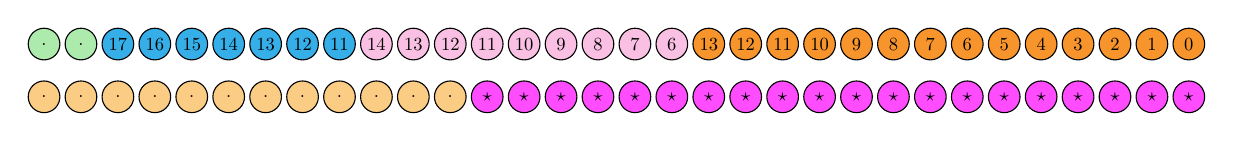
\begin{tikzpicture}[scale=0.67,transform shape]
\draw[fill=LimeGreen!40] (0,0) circle (.3) node{.};
\draw[fill=LimeGreen!40] (0.7,0) circle (.3) node{.};
\draw[fill=Cerulean!85] (1.4,0) circle (.3) node{17};
\draw[fill=Cerulean!85] (2.1,0) circle (.3) node{16};
\draw[fill=Cerulean!85] (2.8,0) circle (.3) node{15};
\draw[fill=Cerulean!85] (3.5,0) circle (.3) node{14};
\draw[fill=Cerulean!85] (4.2,0) circle (.3) node{13};
\draw[fill=Cerulean!85] (4.9,0) circle (.3) node{12};
\draw[fill=Cerulean!85] (5.6,0) circle (.3) node{11};
\draw[fill=Rhodamine!30] (6.3,0) circle (.3) node{14};
\draw[fill=Rhodamine!30] (7.0,0) circle (.3) node{13};
\draw[fill=Rhodamine!30] (7.7,0) circle (.3) node{12};
\draw[fill=Rhodamine!30] (8.4,0) circle (.3) node{11};
\draw[fill=Rhodamine!30] (9.1,0) circle (.3) node{10};
\draw[fill=Rhodamine!30] (9.8,0) circle (.3) node{ 9};
\draw[fill=Rhodamine!30] (10.5,0) circle (.3) node{ 8};
\draw[fill=Rhodamine!30] (11.2,0) circle (.3) node{ 7};
\draw[fill=Rhodamine!30] (11.9,0) circle (.3) node{ 6};
\draw[fill=BurntOrange!85] (12.6,0) circle (.3) node{13};
\draw[fill=BurntOrange!85] (13.3,0) circle (.3) node{12};
\draw[fill=BurntOrange!85] (14.0,0) circle (.3) node{11};
\draw[fill=BurntOrange!85] (14.7,0) circle (.3) node{10};
\draw[fill=BurntOrange!85] (15.4,0) circle (.3) node{ 9};
\draw[fill=BurntOrange!85] (16.1,0) circle (.3) node{ 8};
\draw[fill=BurntOrange!85] (16.8,0) circle (.3) node{ 7};
\draw[fill=BurntOrange!85] (17.5,0) circle (.3) node{ 6};
\draw[fill=BurntOrange!85] (18.2,0) circle (.3) node{ 5};
\draw[fill=BurntOrange!85] (18.9,0) circle (.3) node{ 4};
\draw[fill=BurntOrange!85] (19.6,0) circle (.3) node{ 3};
\draw[fill=BurntOrange!85] (20.3,0) circle (.3) node{ 2};
\draw[fill=BurntOrange!85] (21.0,0) circle (.3) node{ 1};
\draw[fill=BurntOrange!85] (21.7,0) circle (.3) node{ 0};
\draw[fill=YellowOrange!45] (0,-1) circle (.3) node{.};
\draw[fill=YellowOrange!45] (0.7,-1) circle (.3) node{.};
\draw[fill=YellowOrange!45] (1.4,-1) circle (.3) node{.};
\draw[fill=YellowOrange!45] (2.1,-1) circle (.3) node{.};
\draw[fill=YellowOrange!45] (2.8,-1) circle (.3) node{.};
\draw[fill=YellowOrange!45] (3.5,-1) circle (.3) node{.};
\draw[fill=YellowOrange!45] (4.2,-1) circle (.3) node{.};
\draw[fill=YellowOrange!45] (4.9,-1) circle (.3) node{.};
\draw[fill=YellowOrange!45] (5.6,-1) circle (.3) node{.};
\draw[fill=YellowOrange!45] (6.3,-1) circle (.3) node{.};
\draw[fill=YellowOrange!45] (7.0,-1) circle (.3) node{.};
\draw[fill=YellowOrange!45] (7.7,-1) circle (.3) node{.};
\draw[fill=Fuchsia!70] (8.4,-1) circle (.3) node{$\star$};
\draw[fill=Fuchsia!70] (9.1,-1) circle (.3) node{$\star$};
\draw[fill=Fuchsia!70] (9.8,-1) circle (.3) node{$\star$};
\draw[fill=Fuchsia!70] (10.5,-1) circle (.3) node{$\star$};
\draw[fill=Fuchsia!70] (11.2,-1) circle (.3) node{$\star$};
\draw[fill=Fuchsia!70] (11.9,-1) circle (.3) node{$\star$};
\draw[fill=Fuchsia!70] (12.6,-1) circle (.3) node{$\star$};
\draw[fill=Fuchsia!70] (13.3,-1) circle (.3) node{$\star$};
\draw[fill=Fuchsia!70] (14.0,-1) circle (.3) node{$\star$};
\draw[fill=Fuchsia!70] (14.7,-1) circle (.3) node{$\star$};
\draw[fill=Fuchsia!70] (15.4,-1) circle (.3) node{$\star$};
\draw[fill=Fuchsia!70] (16.1,-1) circle (.3) node{$\star$};
\draw[fill=Fuchsia!70] (16.8,-1) circle (.3) node{$\star$};
\draw[fill=Fuchsia!70] (17.5,-1) circle (.3) node{$\star$};
\draw[fill=Fuchsia!70] (18.2,-1) circle (.3) node{$\star$};
\draw[fill=Fuchsia!70] (18.9,-1) circle (.3) node{$\star$};
\draw[fill=Fuchsia!70] (19.6,-1) circle (.3) node{$\star$};
\draw[fill=Fuchsia!70] (20.3,-1) circle (.3) node{$\star$};
\draw[fill=Fuchsia!70] (21.0,-1) circle (.3) node{$\star$};
\draw[fill=Fuchsia!70] (21.7,-1) circle (.3) node{$\star$};
\end{tikzpicture}
\end{center}
\caption{The inter-snippet buffer for steps $\state_{23}$ to $\state_{26}$.
From top to bottom, left to right, the two lime bits (\protect\tikz{\protect\draw[fill=LimeGreen!40] (0,0) circle (.15);})
are bits of padding that do not hold any meaningful data;
bright cerulean (\protect\tikz{\protect\draw[fill=Cerulean!85] (0,0) circle (.15);})
refers to bits from $\expmess_{21}$ and light rhodamine (\protect\tikz{\protect\draw[fill=Rhodamine!30] (0,0) circle (.15);})
to bits from $\expmess_{19}$; bright (burnt) orange (\protect\tikz{\protect\draw[fill=BurntOrange!85] (0,0) circle (.15);})
bits come from $\expmess_{20}$. Light (yellow) orange (\protect\tikz{\protect\draw[fill=YellowOrange!45] (0,0) circle (.15);})
bits are also padding bits, and bright fuchsia (\protect\tikz{\protect\draw[fill=Fuchsia!70] (0,0) circle (.15);})
bits finally hold the index of an extended base solution.}
\label{fig:nb_packing76_2}
\end{figure}

\subsection{An example of colliding message pair}
\label{sec:colli_ex}
We give an example of collision in \autoref{tbl:fscoll76}.
This shows the two (message, \iv) pairs with their (identical) resulting digest. The \ivs and the digests' words are ordered similarly
as in \autoref{tab:sha_iv}; the messages' words are ordered as $\mess_0,\ldots,\mess_{15}$ from top to bottom, left to right.
%The separations between the 32-bit words are materialized with a `\texttt{|}' symbol.
Although the separations between the 32-bit words are not materialized, they should be taken into account, and
the values should not be interpreted as binary strings.
Note that unlike most inputs discussed in this article, the \iv values are compatible with the \emph{original} description
of \shaone, \ie they are not (all) equal to the corresponding state values $\state_{0},\ldots,\state_{-4}$; compared to
$\state_{-2},\ldots,\state_{-4}$, the last three \iv words are rotated by two to the right.

\begin{table}[!htb]
\caption{A freestart collision for 76-step \shaone. Message and \iv bytes with differences are highlighted with \framebox{\color{LimeGreen}coloured boxes}.}\label{tbl:fscoll76}
\centering
\begin{tabular}{c c}
\toprule
 & Message 1\\
\midrule
\iv &  \hspace{-1.95mm}\tt 81 bf 23 06  41 b8 3b \framebox{\color{Cerulean}5c  03} e9 a7 8f  ba 50 28 d5  fc 50 87 88 \\
\midrule
$\mess$ & \tt \hspace{1.15mm}46\hspace{1.25mm} fa 5a \framebox{\color{Cerulean}88  f4} f0 c7 \framebox{\color{Cerulean}f0  b8} de db \framebox{\color{Cerulean}ec  95} 1e 25 \framebox{\color{Cerulean}88}\\
        & \tt \framebox{\color{Cerulean}77} 34 fd \framebox{\color{Cerulean}f5 4c} 42 c4 \framebox{\color{Cerulean}97 52} d7 d8 \framebox{\color{Cerulean}f9 5f} 14 52 \framebox{\color{Cerulean}ea} \\
		& \tt \framebox{\color{Cerulean}b4} 9e 93 \framebox{\color{Cerulean}b2 91} c2 30 \framebox{\color{Cerulean}71 c7} 0f 35 \framebox{\color{Cerulean}9b 8a} ba cf \framebox{\color{Cerulean}af} \\
		& \tt \framebox{\color{Cerulean}b3} 7f fb \framebox{\color{Cerulean}27 3d} fe 7f \framebox{\color{Cerulean}ad 7a} de 56 \framebox{\color{Cerulean}95 20} fd 7c \framebox{\color{Cerulean}ea} \\
\midrule
$\compress(\iv,\mess)$ & \tt af 49 5d 10  52 82 35 03  e4 9e 46 78  dc e7 f3 b3  d6 da a3 24 \\
\bottomrule\\

\toprule
 & Message 2 \\
\midrule
$\diff$\iv & \hspace{-1.95mm}\tt 81 bf 23 06  41 b8 3b \framebox{\color{RubineRed}5d  83} e9 a7 8f  ba 50 28 d5  fc 50 87 88 \\
\midrule
$\diff\mess$ & \tt \hspace{1.15mm}46\hspace{1.25mm} fa 5a \framebox{\color{RubineRed}98  f0} f0 c7 \framebox{\color{RubineRed}ec  7a} de db \framebox{\color{RubineRed}f8  99} 1e 25 \framebox{\color{RubineRed}8a}\\
      		 & \tt \framebox{\color{RubineRed}b7} 34 fd \framebox{\color{RubineRed}e5 f8} 42 c4 \framebox{\color{RubineRed}8b 6e} d7 d8 \framebox{\color{RubineRed}fd e3} 14 52 \framebox{\color{RubineRed}f0} \\
			 & \tt \framebox{\color{RubineRed}94} 9e 93 \framebox{\color{RubineRed}a2 b5} c2 30 \framebox{\color{RubineRed}6d 2b} 0f 35 \framebox{\color{RubineRed}8f 86} ba cf \framebox{\color{RubineRed}ad} \\
			 & \tt \framebox{\color{RubineRed}73} 7f fb \framebox{\color{RubineRed}37 89} fe 7f \framebox{\color{RubineRed}b1 56} de 56 \framebox{\color{RubineRed}91 9c} fd 7c \framebox{\color{RubineRed}f2} \\
\midrule
$\compress(\diff\iv,\diff\mess)$ & \tt af 49 5d 10  52 82 35 03  e4 9e 46 78  dc e7 f3 b3  d6 da a3 24 \\
\bottomrule
\end{tabular}
\end{table}

%\begin{table}[!htb]
%\caption{A freestart collision for 76-step \shaone. Message and \iv bytes with differences are highlighted with \framebox{\color{LimeGreen}coloured boxes}.}\label{tbl:fscoll76}
%\centering
%\begin{tabular}{c c}
%\toprule
% & Message 1\\
%\midrule
%\iv &  \tt 81 bf 23 06 | 41 b8 3b \framebox{\color{Cerulean}5c | 03} e9 a7 8f | ba 50 28 d5 | fc 50 87 88 \\
%\midrule
%$\mess$ & \tt \hspace{1.15mm}46\hspace{1.25mm} fa 5a \framebox{\color{Cerulean}88 | f4} f0 c7 \framebox{\color{Cerulean}f0 | b8} de db \framebox{\color{Cerulean}ec | 95} 1e 25 \framebox{\color{Cerulean}88}\\
%      & \tt \framebox{\color{Cerulean}77} 34 fd \framebox{\color{Cerulean}f5 | 4c} 42 c4 \framebox{\color{Cerulean}97 | 52} d7 d8 \framebox{\color{Cerulean}f9 | 5f} 14 52 \framebox{\color{Cerulean}ea} \\
%			& \tt \framebox{\color{Cerulean}b4} 9e 93 \framebox{\color{Cerulean}b2 | 91} c2 30 \framebox{\color{Cerulean}71 | c7} 0f 35 \framebox{\color{Cerulean}9b | 8a} ba cf \framebox{\color{Cerulean}af} \\
%			& \tt \framebox{\color{Cerulean}b3} 7f fb \framebox{\color{Cerulean}27 | 3d} fe 7f \framebox{\color{Cerulean}ad | 7a} de 56 \framebox{\color{Cerulean}95 | 20} fd 7c \framebox{\color{Cerulean}ea} \\
%\midrule
%$\compress(\iv,\mess)$ & \tt af 49 5d 10 | 52 82 35 03 | e4 9e 46 78 | dc e7 f3 b3 | d6 da a3 24 \\
%\bottomrule\\
%
%\toprule
% & Message 2 \\
%\midrule
%$\diff$\iv & \hspace{-1.95mm}\tt 81 bf 23 06 | 41 b8 3b \framebox{\color{RubineRed}5d | 83} e9 a7 8f | ba 50 28 d5 | fc 50 87 88 \\
%\midrule
%$\diff\mess$ & \tt \hspace{1.15mm}46\hspace{1.25mm} fa 5a \framebox{\color{RubineRed}98 | f0} f0 c7 \framebox{\color{RubineRed}ec | 7a} de db \framebox{\color{RubineRed}f8 | 99} 1e 25 \framebox{\color{RubineRed}8a}\\
%      & \tt \framebox{\color{RubineRed}b7} 34 fd \framebox{\color{RubineRed}e5 | f8} 42 c4 \framebox{\color{RubineRed}8b | 6e} d7 d8 \framebox{\color{RubineRed}fd | e3} 14 52 \framebox{\color{RubineRed}f0} \\
%			& \tt \framebox{\color{RubineRed}94} 9e 93 \framebox{\color{RubineRed}a2 | b5} c2 30 \framebox{\color{RubineRed}6d | 2b} 0f 35 \framebox{\color{RubineRed}8f | 86} ba cf \framebox{\color{RubineRed}ad} \\
%			& \tt \framebox{\color{RubineRed}73} 7f fb \framebox{\color{RubineRed}37 | 89} fe 7f \framebox{\color{RubineRed}b1 | 56} de 56 \framebox{\color{RubineRed}91 | 9c} fd 7c \framebox{\color{RubineRed}f2} \\
%\midrule
%$\compress(\diff\iv,\diff\mess)$ & \tt af 49 5d 10 | 52 82 35 03 | e4 9e 46 78 | dc e7 f3 b3 | d6 da a3 24 \\
%\bottomrule
%\end{tabular}
%\end{table}
